% !TEX root = Ausarbeitung.tex


\section{Einleitung}
\subsection{Projektbeschreibung}
Im Januar 2020 wird in den USA ein Gesetz in Kraft treten. Dieses verpflichtet die Firma Kaersk dazu, alle Schiffscontainer mit einem Tracking-Gerät auszustatten. Dieses Gerät muss die Position des entsprechenden Container über die letzten 9 Monate dokumentieren. Unsere Geräte CONTRAC mit der zugehörigen Software CONSERV bietet diese Möglichkeit. Aus diesem Grund hat uns Kaersk beauftragt die Container des Schiffs "`Event Horizon"' mit unserem System auszustatten. Um die Anforderungen der Firma Kaersk zu erfüllen müssen diese Geräte allerdings mit ZigBee ausgestattet werden und die Software entsprechend erweitert werden. Auch übernehmen wir die Verwaltung des Servers CONSERV für Kaersk.
\section{Annahmen}
\subsection{Sitze und Örtlichkeiten}
\begin{enumerate}
    \item Der Sitz der Firma Echtzeitsysteme GmbH ist Albstadt
    \item Der Sitz der Firma DOTDAT GmbH ist Hamburg
    \item Der bei Kaersk beschäftigte Projektleiter Lars Haekinson arbeitet in Hamburg
    \item Die Firma EZ besitzt einen Vorrat von ca. 100 CONTRAC-Geräten für Test- und Entwicklungszwecke in Albstadt
    \item Der Kunde verlangt keine Änderungen während des Projektzeitraums
   
    \item Die Kosten für die CONTRAC-Geräte enthalten eine Pauschale für eine LTE Verbindung mit einer eingebaut E-Sim.
	\item Die Tochterfirma kann jederzeit, ohne Verzögerungen mit der Produktion beginnen.
    \item Die Lieferung großer Frachten aus Shenzhen dauert 40 Tage und kostet 1.500 Euro pro Container.
    \item Die Lieferung kleiner Mengen per Luftfracht dauert 5 Tage und kostent 20.000 Euro pro Tonne.
    \item Alle Mitarbeiter sind in der angegebenen Zeit für das Projekt verfügbar.
\end{enumerate}

\section{Projektinhalt}
\subsection{Aktivitäten}
\begin{table}[H]
    \renewcommand{\arraystretch}{1.05}
    \begin{center}
        \begin{tabular}{l|l}
            \hline
            \textbf{ID} & \textbf{Aktivität}\\\hline
            A    & Projektmanager\\ \hline
            A1   & Ausführungen\\ \hline
            A2   & Reviews\\ \hline
            A3 & Kommunikation \\\hline
            B    & CONTRAC\\ \hline
            B1   & Entwicklung Verbesserung Hardware (ZigBee und Akku) \\ \hline
            B2.1 & Einkauf der Teile\\\hline
            B2.2 & Produktion beauftragen\\ \hline
            B2.3 & Produktion\\ \hline
            B3 & QS Shenzhen\\ \hline
            B4.1 & Anbauer buchen\\ \hline
            B4.2 & Anbau testen\\ \hline
            B4.3 & Anbau vorstellen\\ \hline
            B4.4 & Anbauer schulen\\ \hline
            B4.5 & Anbau\\ \hline
            C    & CONSERV\\ \hline
            C1.1 & Patch-Software optimieren\\ \hline
            C1.2 & Patch-Software testen \\ \hline
            C1.3 & Patch-Software Fehler beheben\\ \hline
            C1.4   & Mit 5250 Geräten in Shenzhen testen\\ \hline
            C2 & Anpassung Look\&Feel\\\hline
            C3.1 & Cloud-Anbieter suchen \\ \hline
            C3.2 & Cloud einrichten      \\ \hline
            C3.3 & Server einrichten     \\ \hline
            D    & CONTRAC-Firmware      \\ \hline
            D1   & ZigBee einbauen       \\ \hline
            D2.1 & Patch-Funktion optimieren \\ \hline
            D2.2 & Patch-Funktion testen \\ \hline
            D2.3 & Patch-Funktion Fehler beheben  \\
        \end{tabular}
        \caption{Aktivitäten im Projekt}
    \end{center}
\end{table}

\subsection{Work-Breakdown-Strukture}
\begin{figure}[H]
    \begin{center}
        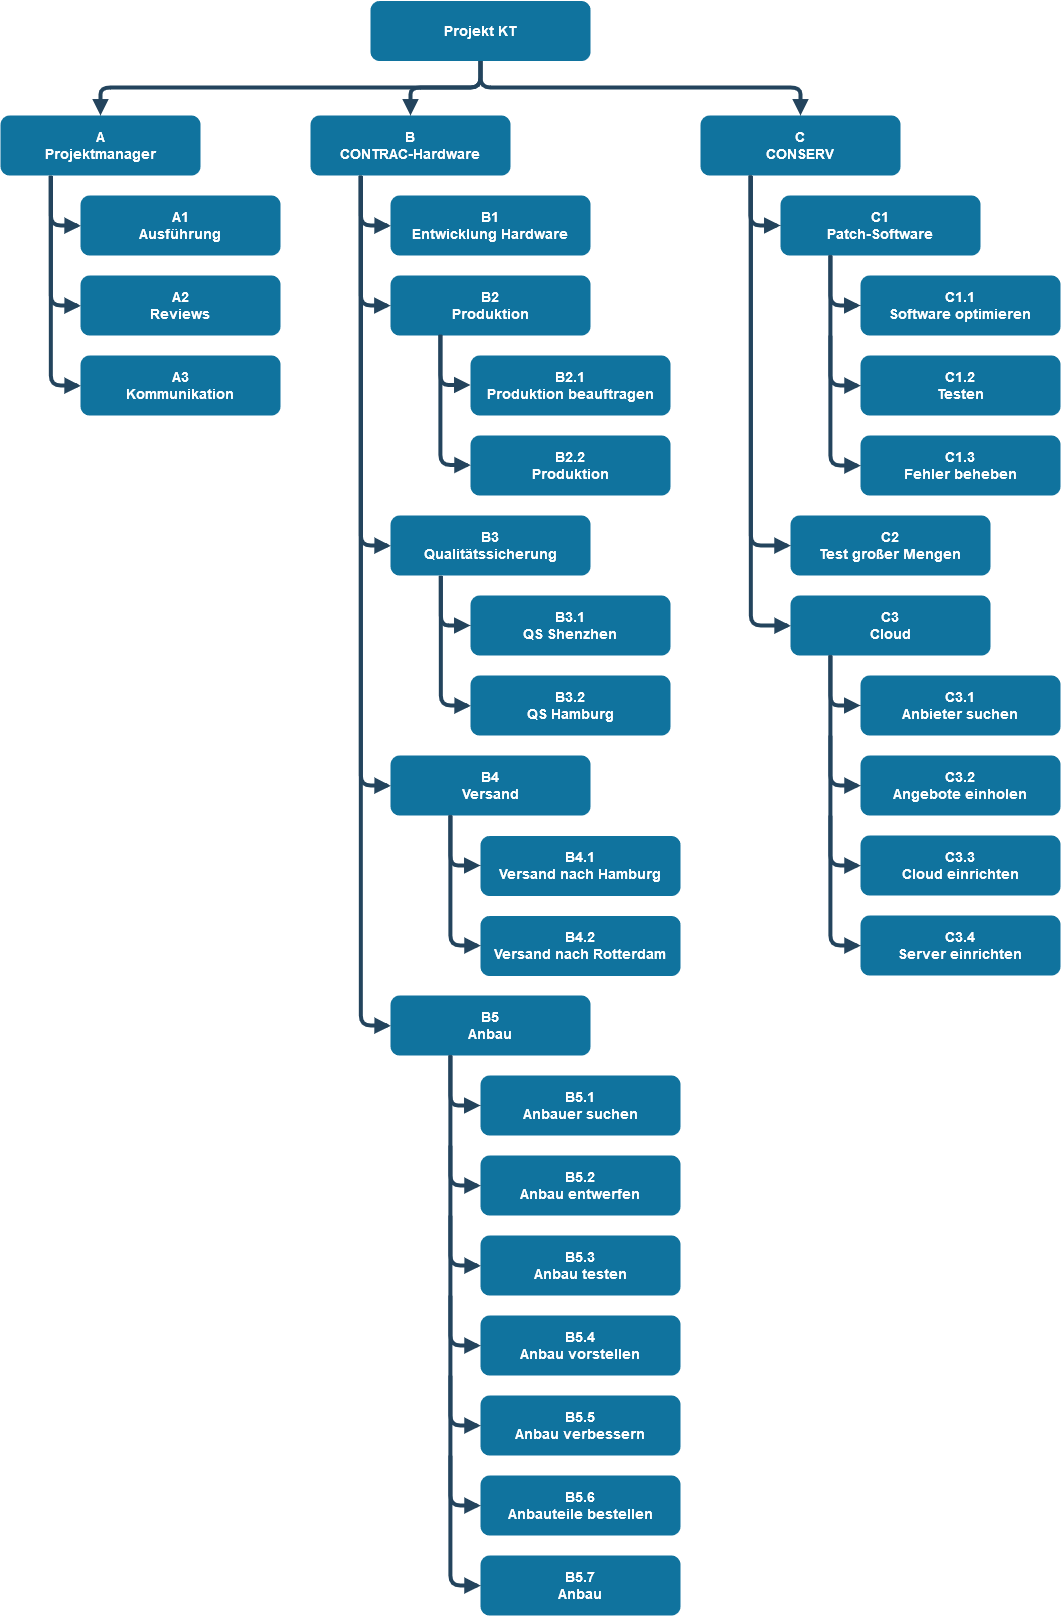
\includegraphics[width=0.8\textwidth]{WBS.png}
    \end{center}
    \caption{Work-Breakdown-Strukture}
\end{figure}
\subsection{Oranisation Breakdown Strukture}
\begin{figure}[H]
    \begin{center}
        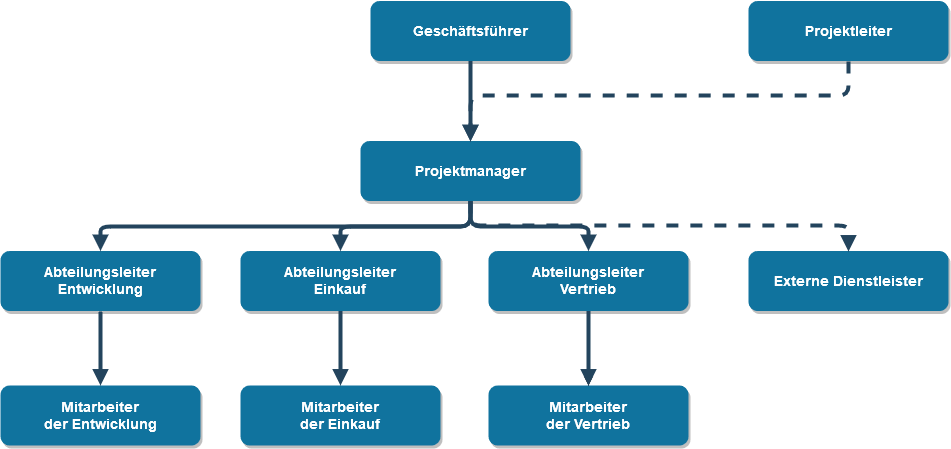
\includegraphics[width=0.8\textwidth]{OBS.png}
    \end{center}
    \caption{Organisation-Breakdown-Strukture}
\end{figure}
\section{Zeitmanagement}
\subsection{Aktivitätendauer}

\begin{table}[H]
	\renewcommand{\arraystretch}{1.05}
	\begin{center}
		\begin{tabular}{l|l|l}
			\hline
			\textbf{ID} & \textbf{Aktivität} & \textbf{Dauern in Tagen}\\\hline
			A    & Projektmanager &  \\ \hline
			A1   & Ausführungen & 70 \\  \hline
			A2   & Reviews & 20 \\ \hline
			A3 & Kommunikation & 20 \\\hline
			B    & CONTRAC & \\ \hline
			B1   & Entwicklung Verbesserung Hardware (ZigBee und Akku) & 20\\ \hline
			B2.1 & Einkauf der Teile & 5\\\hline
			B2.2 & Produktion beauftragen & 5\\ \hline
			B2.3 & Produktion & 30\\ \hline
			B3 & QS Shenzhen & 20\\ \hline
			B4.1 & Anbauer buchen & 5\\ \hline
			B4.2 & Anbau testen &5\\ \hline
			B4.3 & Anbau vorstellen &3\\ \hline
			B4.4 & Anbauer schulen &1\\ \hline
			B4.5 & Anbau &3\\ \hline
			C    & CONSERV &\\ \hline
			C1.1 & Patch-Software optimieren & 20\\ \hline
			C1.2 & Patch-Software testen  & 15 \\ \hline
			C1.3 & Patch-Software Fehler beheben  & 10\\ \hline
			C1.4  & Mit 5250 Geräten in Shenzhen testen  & 5\\ \hline
			C2 & Anpassung Look\&Feel  & 10\\\hline
			C3.1 & Cloud-Anbieter suchen  & 2\\ \hline
			C3.2 & Cloud einrichten       & 5\\ \hline
			C3.3 & Server einrichten      & 5\\ \hline
			D    & CONTRAC-Firmware      & \\ \hline
			D1   & ZigBee einbauen       & 10 \\ \hline
			D2.1 & Patch-Funktion optimieren & 20 \\ \hline
			D2.2 & Patch-Funktion testen & 20 \\ \hline
			D2.3 & Patch-Funktion Fehler beheben  & 10 \\
		\end{tabular}
		\caption{Dauer der Aktivitäten im Projekt}
	\end{center}
\end{table}

\subsection{Meilensteine}

\textbf{M1: Kick-Off}\\
\textbf{M2: Patch-Update Funktion funktionstüchtig} Die Patch-Update Funktion wurde erfolgreich getestet und die dementsprechende Entwicklung ist abgeschlossen.\\
\textbf{M3: CONTRAC-Firmware um ZigBee ergänzt} Die Firmware für die CONTRAC-Geräte wurde für ZigBee ergänzt und erfolgreich getestet.\\
\textbf{M4: Hardware-Entwicklung abgeschlossen} Die Entwicklung der Hardware mit den Ergänzungen um ZigBee und größeren Akku ist abgeschlossen.\\
\textbf{M5: Produktion in Shenzhen beauftragt} Die Produktion der Geräte in Shenzhen wurde in Auftrag gegeben.\\
\textbf{M6: CONSERV-Server mit 5250 Geräten getestet} Der CONSERV-Server wurde mit 5250 erfolgreich getestet.\\
\textbf{M7: QS Shenzhen erfolgreich} Alle produzierten Geräte haben die Qualiätssicherung in Shenzhen erfolgreich bestanden.\\
\textbf{M8: Geräte aus Shenzhen empfangen} Die Geräte aus Shenzhen sind unbschadet in Rotterdam angekommen.\\
\textbf{M9: Montage von KT abgenommen} Der Montagevorgang wurde von Kaersk abgenommen.\\
\textbf{M10: Geräte montiert} Die Geräte wurden alle an den Containern montiert.\\
\textbf{M11: Inbetriebnahme} Alle Geräte wurden problemlos in Betrieb genommen.\\
\textbf{M12: Support/Hosting beendet}

\subsection{PERT} % Kritischer Pfad !

\subsection{Gant} % Kritischer Pfad !

\section{Kommunikationsplan}
\subsection{Beteiligte}
\begin{table}[H]
    \renewcommand{\arraystretch}{1.1}
    \begin{center}
        \begin{tabular}{l|l}
            \textbf{Stakeholder} & \textbf{Kürzel}\\\hline
            Vertreter DOTDAT & \\
            Projektmanager & PM\\
            Lars & LH\\
            
            
            
            
            
        \end{tabular}
    \end{center}
    \caption{Stakeholder}
\end{table}
\subsection{Geplante Meetings}
 
\subsubsection{Kickoff}
\textbf{Wann:} \\
\textbf{Wer:} PM, LH, Vertreter von Kaersk\\
\textbf{Wo:} Albstadt, EZ\\
\textbf{Wie oft:} Einmalig\\
\textbf{Produzierte Dokumente:} Protokoll


\subsubsection{Dayly EZ}
\textbf{Wann:} 9:00 Uhr\\
\textbf{Wer:} Alle beteiligten Entwickler, PM\\
\textbf{Wo:} Albstadt, EZ, Entwicklungsbüro\\
\textbf{Wie oft:}Täglich\\
\textbf{Produzierte Dokumente:} Protokoll

\subsubsection{Weekly Review}
\textbf{Wann:}  Donnerstags, 14:00\\
\textbf{Wer:} LH, PM , alle beteiligten Entwickler, DotDat\\
\textbf{Wo:}Albstadt, EZ, Entwicklungsbüro\\
\textbf{Wie oft:} Wöchentlich\\
\textbf{Produzierte Dokumente:} Protokoll, Report

\subsubsection{Präsentation der Befestigung}
\textbf{Wann:} \\
\textbf{Wer:} PM, LH, Vertreter von Kaersk\\
\textbf{Wo:} Hamburg, Kaersk\\
\textbf{Wie oft:} Einmalig\\
\textbf{Produzierte Dokumente:} Protokoll, schriftliche Beschreibung der Befestigung, schriftliche Zusage von Maersk

\subsection{Reports}
Sämtliche Berichte werden im firmeneigenen Confluence gesammelt und allen Beteiligten zur Verfügung gestellt.

\subsubsection{Template für Reports}

\begin{table}[H]
	\renewcommand{\arraystretch}{1.4}
	\begin{center}
		\begin{tabular}{|l|l|l|}\hline
			\textbf{Projekt} & \multicolumn{2}{l|}{KT-CVF }\\\hline
			\textbf{Datum} &\multicolumn{2}{l|}{} \\ \hline
			& Bewertung (1-7) & Details?\\\hline
			\textbf{Arbeitsumfang} && \qquad\qquad\qquad\qquad\\\hline
			\textbf{Fortschritt} && \\\hline
			\textbf{Arbeitsklima} & &\\\hline
			\textbf{Kommunikation} & &\\\hline
		\end{tabular}
	\end{center}
\end{table}

\section{Qualität}
\subsection{Qualitätsprozesse}
Um die Qualität der Hardware und Software werden bei EZ verschieden Prozesse eingesetzt. Dazu gehört eine doppelte Qualitätskontrolle der Hardware, Code Reviews sowie ausführliche und automatisierte Tests für die Software.
\subsection{Qualitätskontrolle der Hardware}
Alle CONTRAC-Geräte werden in Shenzhen und in Hamburg durch eine elektrische Kontrolle auf ihre Funktionalität geprüft.
\subsubsection{Code Review}
Jeder Code muss vor dem Mergen in den master-Branch durch einen zweiten Entwickler getestet und kontrolliert werden.
\subsubsection{Unit Test}
Für jede Softwarekomponente muss ein Unit-Test erstellt werden, der vor jedem Einchecken erfolgreich durchgeführt werden muss. Auch der Build-Server des Continuous-Integration-Zyklus muss die Tests erfolgreich ausführen. Bei einem Fehlschlag muss dieser zeitnah behoben werden.
\subsubsection{Test}
Jede erstellte Komponente muss vom Entwickler ausführlich getestet werden. Jede Komponente muss auch von einem zweiten Mitarbeiter getestet werden.
\subsection{Ticketsytem}
Als Ticktsystem kommt das firmeneigene Jira zum Einsatz. Dieses ist über die Adresse \texttt{https://jira.ez.de} verfügbar. Alle Entwickler und Product Owner besitzen ein Zugang zu diesem System.
\subsection{Versionierungssystem}
Als Versionierungssystem für das Projekt wird Git eingesetzt. Dieses ist allen Entwicklern auf ihren Computern verfügbar. Als Git-Remote dient der firmeneigene Bitbucket-Server, der unter der Adresse \texttt{git.ez.de} verfügbar ist. Auch aus dem Internet ist der Server unter dieser Adresse verfügbar.

Eine Commit-Message muss immer die getätigte Arbeit beschreiben und eine eindeutige Zuordung zu einem Ticket oder ein User Story ermöglichen. Dazu werden diese über ihre eindeutige Bezeichnung (US-3, BUG-5) erwähnt.
\subsection{Codestyle}
Der geschriebene Code muss den Stylerichtlinien der Firma entsprechen. Diese können dem hausinternen Wiki unter \texttt{wiki.ez.de} entnommen werden. Konfigurationsdateien für verschiedene IDEs und Formatierer können dort auch heruntergeladen werden. Diese Richtlinien werden auch an externe Firmen weitergegeben. 
\subsection{Bugverlauf}
Jeder entdeckte Bug muss in Jira dokumentiert werden. Die Bugs fließen dann in die Backlogs für die Entwicklung ein. Dort werden sie mit erhöhter Priorität belegt.
Für die Behebung des Fehlers wird der Bug reporduziert und der Bug in einem Bugfix-Branch korrigiert. Dieser wird dann in den aktuellen Branch gemergt.


\subsection{Befestigung des Gerät CONTRAC}
Das Gerät CONTRAC muss am 15. Oktober innerhalb von 72h an 5000 Containern befestigt werden.

Die Geräte werden an den Containern mit Spezialkleber befestigt. Der Kleber wird von der Firma Sika hergestellt und regulär für das Verkleben von Fahrzeugkarosserien verwendet. Er wir dort als Ersatz von Schweißnähten genutzt und hält großen Belastungen und Temperaturschwankungen stand.\\
Die Montage wird von Zweierteams durchgeführt. Dieses reinigt zuerst mit einem sich verflüchtigendem Reinigungsmittel die Montagestelle am Container. Dann wird ein CONTRAC-Geräte in das Aufpresswerkzeug gesetzt. Der Kleber wird mit einer Spritze aufgetragen, das Gerät an den Container angepresst und anschließend angeschaltet. Dieser Vorgang kann in 2 Minuten durchgeführt werden. Die Arbeiter stehen für die Montage auf einer erhöhten Fläche, um den Montagepunkt leichter zu erreichen. Das Aufpresswerkzeug besitzt wie ein Drehmomentschlüssel einen Auslösemechanismus um den optimalen Druck zu gewährleisten.

Für die Montage in Rotterdam werden externe Mitarbeiter akquiriert, die diese Arbeit unter Aufsicht durchführen. Diese werden am Tag vor der Montage geschult. Die Montage findet an 6 Containerbrücken statt. Da für die Verladung eines Containers ca. 3,2\,min benötigt werden, dauert die Montage entsprechend 45 Stunden. In dieser Zeit wechseln sich Zweierteams im Dreischichtbetrieb ab. Damit sind für die Montage 36 Arbeiter notwendig.


\section{Risikoplan}
\subsection{Annahmen} % Auswahl

\textbf{Änderungen während der Projektlaufzeit}\\
\textbf{Die Tochterfirma kann nicht rechtzeitig mit der Produktion beginnen}\\
\textbf{Die Lieferung der Geräte dauert länger als vorgesehen}

\subsection{Risiken mit Priorität} %3 Stück

Die drei wichtigsten Risiken sind die folgenden:
\begin{enumerate}
	\item \textbf{R1: Änderungen während der Projektlaufzeit:} Der Kunde wünscht Änderungen während der Projektlaufzeit, die die Entwicklung oder Produktion verzögern können.
 	\item \textbf{R2: Verlust der Geräte bei Versand:} Die Geräte gehen beim Versand verloren oder während stark beschädigt. Dann müsste neu produziert und versand werden. Dadurch verzögert sich die Bereitstellung der Geräte. Dies kann bis zur Nichterfüllbarkeit des Zeitlimits führen.
	\item \textbf{R3: Gerätekomponente nicht mehr verfügbar:} Eine geplante Gerätekomponente ist zu Produktionsbeginn nicht verfügbar. Diese muss durch eine andere, funktional gleiche aber teurere Komponente ersetzt werden.
\end{enumerate}


\subsection{Bewertung }
Die Bewertung des Schadens wird wie folgt gestaffelt:	
\begin{table}[H]
	    \renewcommand{\arraystretch}{1.2}
	\begin{center}
	\begin{tabular}{p{2.2cm}|p{2cm}|p{2cm}|p{2cm}|p{2cm}|l}
		
		Projektziel & 0,1 & 0,3 & 0,5 & 0,7 & 0,9 \\\hline
		Kosten & nicht signifikant & \textless{}5\% des Projekt & 5-10\% & 10-20\% & \textgreater{}20\% \\\hline
		Zeitplan & nicht signifikant & \textless{}5\% des Projekt & 5-10\% & 10-20\% & \textgreater{}20\% \\\hline
		Projektinhalt & Kaum betroffen & Kleine Inhalte betroffen & Wichtige Inhalte betroffen & Inhalt für Kunde inaktzeptabel & Fehlentwicklung \\\hline
		Qualität & Kaum Abstriche & kleinere Abstriche & Abstriche & Qualität nicht aktzeptabel & Fehlentwicklung
	\end{tabular}
\end{center}
\end{table}

Daraus lässt sich die folgende Risikomatrix abbilden:
\begin{table}[H]
	\renewcommand{\arraystretch}{1.2}
	\begin{center}
		\begin{tabular}{p{4cm}|c|c|c|c|c}
			
			Schaden in Euro / Wahrscheinlichkeit & 1.000 & 10.000 & 100.000 & 1.000.000 & 10.000.000\\\hline
			0,9 & C & D & D & D & D\\\hline
			0,7 & C & C & D & D & D\\\hline
			0,5 & B & C & C & D & D\\\hline
			0,3 & A & B & B & C &  D\\\hline
			0,1 & A & A & B &  C& D \\\hline
		\end{tabular}
	\end{center}
\end{table}


\subsubsection{R1: Änderungen während der Projektlaufzeit}
\begin{enumerate}
\item \textbf{Schaden}: (bei nichterfüllung des Zeitlimits) > 5.000.000
\item \textbf{Wahrscheinlichkeit}: 0.3
\item \textbf{Klassifizierung}: C
\item \textbf{Gegenmaßnahmen}: Um den Kunden nicht zu verärgern dürfen Änderungen nicht abgelehnt werden. Für diese muss allerdings ein neuer Vertrag abgeschlossen werden, der eine mögliche Veränderung der Projektzeit beinhaltet. Auch können die Änderungen des Kunden bei Bedarf auf einen späteren Zeitpunkt verschoben werden.
\end{enumerate}

\subsubsection{R2: Verlust der Geräte bei Versand}
\begin{enumerate}
	\item \textbf{Schaden}: (bei nichterfüllung des Zeitlimits) > 5.000.000
	\item \textbf{Wahrscheinlichkeit}: 0.1
	\item \textbf{Klassifizierung}: C
	\item \textbf{Gegenmaßnahmen}: Der Versand über eine namenhafte Spedition mit entsprechenden Versicherungen minimiert die Wahrscheinlichkeit und den Schaden.
\end{enumerate}
\subsubsection{R3: Gerätekomponente nicht mehr verfügbar}
\begin{enumerate}
	\item \textbf{Schaden}: 20.000
	\item \textbf{Wahrscheinlichkeit}: 0.3
	\item \textbf{Klassifizierung}: B
	\item \textbf{Gegenmaßnahmen}: Bereits bei der Entwicklung kann eine Komponente gewählt werden, deren Unverfügbarkeit unwahrscheinlicher ist und sich die Verfügbarkeit von einem Händler bestätigen lassen.
\end{enumerate}

\subsection{Risikokosten}

Die Kosten für die Risiken betragen sich damit auf:

\textbf{R1: Änderungen während der Projektlaufzeit} Klasse C  $\rightarrow$ 40.000 Euro\\
\textbf{R2: Verlust der Geräte bei Versand} Klasse C  $\rightarrow$ 50.000 Euro\\
\textbf{R3: Gerätekomponente nicht mehr verfügbar} Klasse B  $\rightarrow$ 6000 Euro\\
\textbf{Summe:} 96.000 Euro

\section{Human Ressources}
\subsection{Aufgabenverteilung}


\begin{table}[H]
	\renewcommand{\arraystretch}{1.05}
	\begin{center}
		\begin{tabular}{l|l|l}
			\hline
			\textbf{ID} & \textbf{Aktivität} & \textbf{Dauern in Tagen}\\\hline
			A    & Projektmanager &  \\ \hline
			A1   & Ausführungen & 70 \\  \hline
			A2   & Reviews & 20 \\ \hline
			A3 & Kommunikation & 20 \\\hline
			B    & CONTRAC & \\ \hline
			B1   & Entwicklung Verbesserung Hardware (ZigBee und Akku) & 20\\ \hline
			B2.1 & Einkauf der Teile & 5\\\hline
			B2.2 & Produktion beauftragen & 5\\ \hline
			B2.3 & Produktion & 30\\ \hline
			B3 & QS Shenzhen & 20\\ \hline
			B4.1 & Anbauer buchen & 5\\ \hline
			B4.2 & Anbau testen &5\\ \hline
			B4.3 & Anbau vorstellen &3\\ \hline
			B4.4 & Anbauer schulen &1\\ \hline
			B4.5 & Anbau &3\\ \hline
			C    & CONSERV &\\ \hline
			C1.1 & Patch-Software optimieren & 20\\ \hline
			C1.2 & Patch-Software testen  & 15 \\ \hline
			C1.3 & Patch-Software Fehler beheben  & 10\\ \hline
			C1.4  & Mit 5250 Geräten in Shenzhen testen  & 5\\ \hline
			C2 & Anpassung Look\&Feel  & 10\\\hline
			C3.1 & Cloud-Anbieter suchen  & 2\\ \hline
			C3.2 & Cloud einrichten       & 5\\ \hline
			C3.3 & Server einrichten      & 5\\ \hline
			D    & CONTRAC-Firmware      & \\ \hline
			D1   & ZigBee einbauen       & 10 \\ \hline
			D2.1 & Patch-Funktion optimieren & 20 \\ \hline
			D2.2 & Patch-Funktion testen & 20 \\ \hline
			D2.3 & Patch-Funktion Fehler beheben  & 10 \\
		\end{tabular}
		\caption{Aufgabenverteilung der Aktivitäten im Projekt}
	\end{center}
\end{table}

\subsection{Motivation} % Teamevents, Awards .. (kostet Geld)
\subsubsection{Abschlussevent} Zum Abschluss des Projekt sind alle Beteiligten zu einer Hafenrundführung und gemeinsamen Essen in Rotterdam eingeladen.
\subsubsection{Zuschlag für außerörtliche Aktivitäten} Für alle Aktivitäten die abseits des Firmensitzes in Albstadt stattfinden erhalten die Mitarbeiter einen Zuschlag. Auch werden natürlich alle Reisekosten erstattet.

\section{Beschaffung} % UserStories an extenern Firma
\subsection{Entwicklung der Hardware bei DOTDAT}
Bei der Firma DOTDAT GmbH wird die Entwicklung der Hardware eingekauft. Die von DOTDAT angefragten UserStories lauten wie folgt:

\textbf{US-DD-1:} Ich als Projektmanager möchte, dass die CONTRAC-Geräte über ZigBee untereinander kommunizieren, sodass diese Daten austauschen können.
\textbf{US-DD-2:} Ich als Projektmanager möchte, dass die CONTRAC-Geräte einen größeren Akku erhalten, sodass sie dauerhaft in Betrieb bleiben können.
\textbf{US-DD-3:} Ich als Projektmanager möchte, dass die CONTRAC-Geräte nicht zu groß werden, sodass sie in das vorgegeben Gehäuse passen
\textbf{US-DD-4:} Ich als Projektmanager möchte, dass die CONTRAC-Geräte erschütterungssicher sind, sodass sie beim Be- und Entladen nicht beschädigt werden.

\subsection{Produktion der Geräte in einer Tochterfirma}
Die Produktion der CONTRAC-Geräte wird bei der Tochterfirma in Shenzhen in Auftrag gegeben. Diese benötigen für die Produktion 30 Tage.

\subsection{Material für den Anbau}
Der Kleber wird direkt beim Hersteller bestellt und an den Standort Albstadt geliefert. Zur Montage wird er nach Rotterdam versand. Die Anpresswerkzeuge können von ansässigen Werkzeugproduzenten gefertigt werden.

\subsection{Helfer für den Anbau}
Die Helfer für den Anbau werden in Rotterdam angeworben. Hier wird über einen Personaldienstleister, der die nötigen Arbeiter zur Verfügung stellen kann, ein Vertrag ausgehandelt.

\subsection{Cloudanbieter für das Hosting}
Der Cloudanbieter für das Hosting muss eine bekannten Serverstandort anbieten und dieser muss innerhalb der Europäischen Union liegen. Er muss alle notwendigen Voraussetzungen für CONSERV erfüllen.


\section{Kostenmanagement}

\subsection{Kostenschätzung}
\subsection{Personalkosten} % Awards, Reise, Hotel, Betriebssätze ...
\subsection{Reisekosten}
% Hotel 100€/Nacht
% 
\subsection{Materialkosten}
% + Versand
\subsection{Risikokosten}
%960000
\subsection{Gewinnmarge}

\subsection{Kontigenz} %

\subsection{Plankosten}






